\documentclass{standalone}
\usepackage{tikz}
\usetikzlibrary{patterns, positioning}

\begin{document}
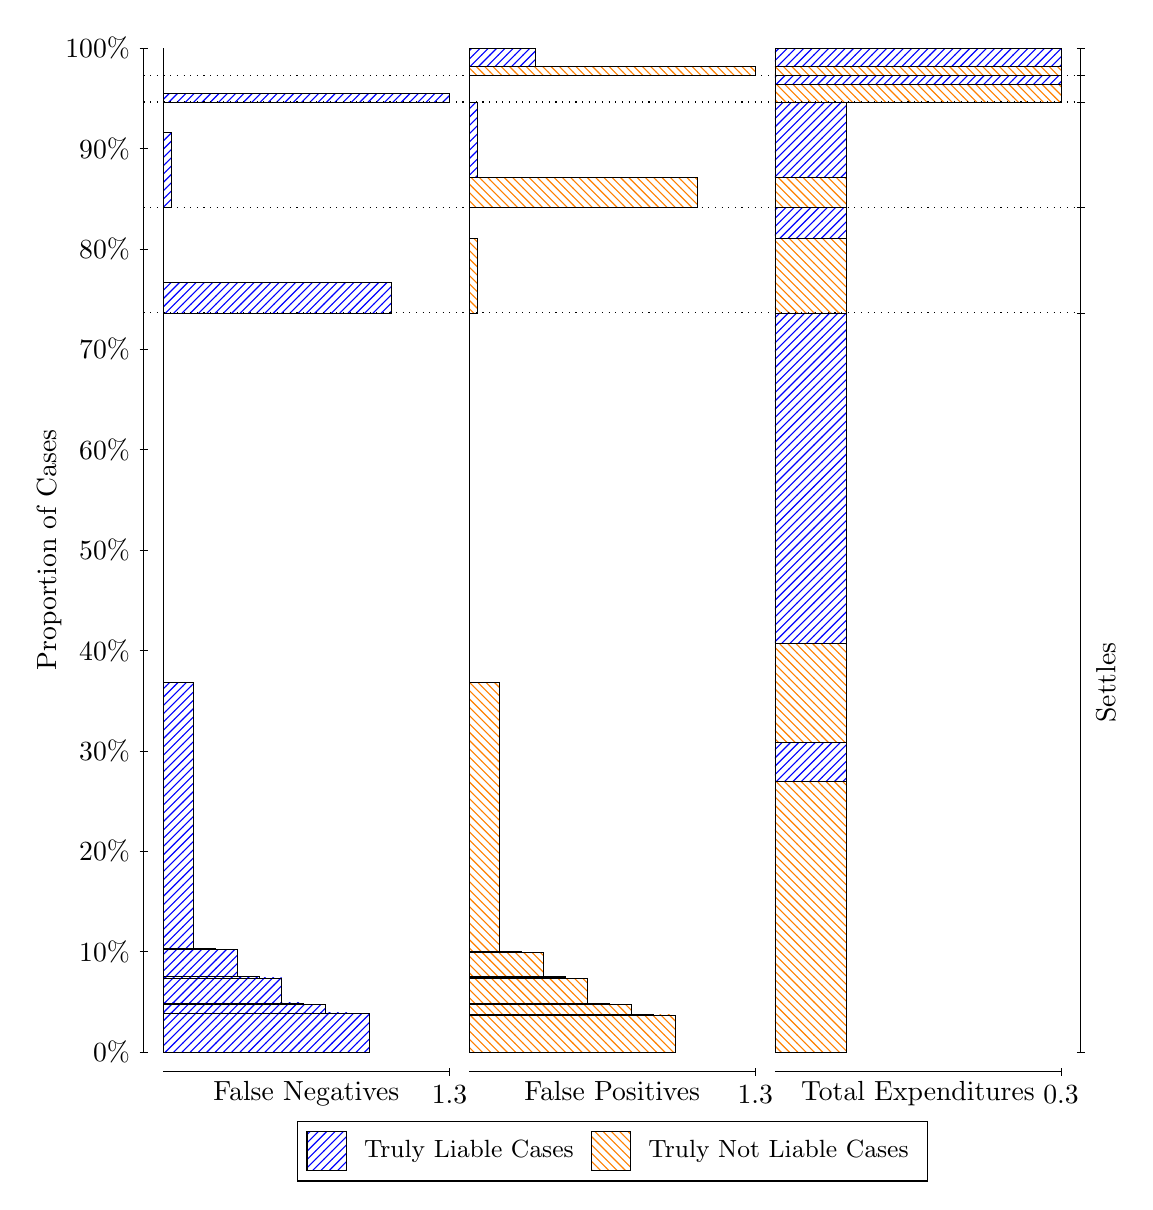
\begin{tikzpicture}
\draw[black, very thin] (1.5,1.75) -- (1.5,14.5);
\node[rotate=90, anchor=center] at (0.3, 8.125) {Proportion of Cases};
\draw[black, very thin] (1.45,1.75) -- (1.55,1.75);
\node[anchor=east] at (1.45, 1.75) {0\%};
\draw[black, very thin] (1.45,3.025) -- (1.55,3.025);
\node[anchor=east] at (1.45, 3.025) {10\%};
\draw[black, very thin] (1.45,4.3) -- (1.55,4.3);
\node[anchor=east] at (1.45, 4.3) {20\%};
\draw[black, very thin] (1.45,5.575) -- (1.55,5.575);
\node[anchor=east] at (1.45, 5.575) {30\%};
\draw[black, very thin] (1.45,6.85) -- (1.55,6.85);
\node[anchor=east] at (1.45, 6.85) {40\%};
\draw[black, very thin] (1.45,8.125) -- (1.55,8.125);
\node[anchor=east] at (1.45, 8.125) {50\%};
\draw[black, very thin] (1.45,9.4) -- (1.55,9.4);
\node[anchor=east] at (1.45, 9.4) {60\%};
\draw[black, very thin] (1.45,10.675) -- (1.55,10.675);
\node[anchor=east] at (1.45, 10.675) {70\%};
\draw[black, very thin] (1.45,11.95) -- (1.55,11.95);
\node[anchor=east] at (1.45, 11.95) {80\%};
\draw[black, very thin] (1.45,13.225) -- (1.55,13.225);
\node[anchor=east] at (1.45, 13.225) {90\%};
\draw[black, very thin] (1.45,14.5) -- (1.55,14.5);
\node[anchor=east] at (1.45, 14.5) {100\%};

\draw[black, very thin] (13.4,1.75) -- (13.4,14.5);
\draw[black, very thin] (13.35,1.75) -- (13.45,1.75);
\node[anchor=west] at (13.35, 1.75) {};
\draw[black, very thin] (13.35,11.137) -- (13.45,11.137);
\node[anchor=west] at (13.35, 11.137) {};
\draw[black, very thin] (13.35,12.472) -- (13.45,12.472);
\node[anchor=west] at (13.35, 12.472) {};
\draw[black, very thin] (13.35,13.814) -- (13.45,13.814);
\node[anchor=west] at (13.35, 13.814) {};
\draw[black, very thin] (13.35,14.156) -- (13.45,14.156);
\node[anchor=west] at (13.35, 14.156) {};
\draw[black, very thin] (13.35,14.5) -- (13.45,14.5);
\node[anchor=west] at (13.35, 14.5) {};

\draw[black, very thin, pattern color=blue, pattern=north east lines] (1.75,1.75) rectangle (4.3702,2.2375);
\draw[black, very thin, pattern color=blue, pattern=north east lines] (1.75,2.2375) rectangle (4.0907,2.2458);
\draw[black, very thin, pattern color=blue, pattern=north east lines] (1.75,2.2458) rectangle (3.8112,2.3585);
\draw[black, very thin, pattern color=blue, pattern=north east lines] (1.75,2.3585) rectangle (3.5317,2.3721);
\draw[black, very thin, pattern color=blue, pattern=north east lines] (1.75,2.3721) rectangle (3.2522,2.6901);
\draw[black, very thin, pattern color=blue, pattern=north east lines] (1.75,2.6901) rectangle (2.9728,2.7132);
\draw[black, very thin, pattern color=blue, pattern=north east lines] (1.75,2.7132) rectangle (2.6933,3.0545);
\draw[black, very thin, pattern color=blue, pattern=north east lines] (1.75,3.0545) rectangle (2.4138,3.0694);
\draw[black, very thin, pattern color=blue, pattern=north east lines] (1.75,3.0694) rectangle (2.1343,6.4392);
\draw[black, very thin, pattern color=orange, pattern=north west lines] (1.75,6.4392) rectangle (1.75,11.137);
\draw[black, very thin, pattern color=blue, pattern=north east lines] (1.75,11.137) rectangle (4.6497,11.523);
\draw[black, very thin, pattern color=orange, pattern=north west lines] (1.75,11.523) rectangle (1.75,12.472);
\draw[black, very thin, pattern color=blue, pattern=north east lines] (1.75,12.472) rectangle (1.8548,13.428);
\draw[black, very thin, pattern color=orange, pattern=north west lines] (1.75,13.428) rectangle (1.75,13.814);
\draw[black, very thin, pattern color=blue, pattern=north east lines] (1.75,13.814) rectangle (5.3833,13.928);
\draw[black, very thin, pattern color=orange, pattern=north west lines] (1.75,13.928) rectangle (1.75,14.156);
\draw[black, very thin, pattern color=orange, pattern=north west lines] (1.75,14.156) rectangle (1.75,14.27);
\draw[black, very thin, pattern color=blue, pattern=north east lines] (1.75,14.27) rectangle (1.75,14.5);
\draw[black, very thin, pattern color=orange, pattern=north west lines] (5.6333,1.75) rectangle (8.2535,2.2215);
\draw[black, very thin, pattern color=orange, pattern=north west lines] (5.6333,2.2215) rectangle (7.974,2.23);
\draw[black, very thin, pattern color=orange, pattern=north west lines] (5.6333,2.23) rectangle (7.6946,2.355);
\draw[black, very thin, pattern color=orange, pattern=north west lines] (5.6333,2.355) rectangle (7.4151,2.3689);
\draw[black, very thin, pattern color=orange, pattern=north west lines] (5.6333,2.3689) rectangle (7.1356,2.6861);
\draw[black, very thin, pattern color=orange, pattern=north west lines] (5.6333,2.6861) rectangle (6.8561,2.6942);
\draw[black, very thin, pattern color=orange, pattern=north west lines] (5.6333,2.6942) rectangle (6.8561,2.7093);
\draw[black, very thin, pattern color=orange, pattern=north west lines] (5.6333,2.7093) rectangle (6.5766,3.0149);
\draw[black, very thin, pattern color=orange, pattern=north west lines] (5.6333,3.0149) rectangle (6.2971,3.0288);
\draw[black, very thin, pattern color=orange, pattern=north west lines] (5.6333,3.0288) rectangle (6.0176,6.4479);
\draw[black, very thin, pattern color=blue, pattern=north east lines] (5.6333,6.4479) rectangle (5.6333,11.137);
\draw[black, very thin, pattern color=orange, pattern=north west lines] (5.6333,11.137) rectangle (5.7381,12.086);
\draw[black, very thin, pattern color=blue, pattern=north east lines] (5.6333,12.086) rectangle (5.6333,12.472);
\draw[black, very thin, pattern color=orange, pattern=north west lines] (5.6333,12.472) rectangle (8.533,12.858);
\draw[black, very thin, pattern color=blue, pattern=north east lines] (5.6333,12.858) rectangle (5.7381,13.814);
\draw[black, very thin, pattern color=orange, pattern=north west lines] (5.6333,13.814) rectangle (5.6333,14.041);
\draw[black, very thin, pattern color=blue, pattern=north east lines] (5.6333,14.041) rectangle (5.6333,14.156);
\draw[black, very thin, pattern color=orange, pattern=north west lines] (5.6333,14.156) rectangle (9.2667,14.27);
\draw[black, very thin, pattern color=blue, pattern=north east lines] (5.6333,14.27) rectangle (6.4718,14.5);
\draw[black, very thin, pattern color=orange, pattern=north west lines] (9.5167,1.75) rectangle (10.425,5.183);
\draw[black, very thin, pattern color=blue, pattern=north east lines] (9.5167,5.183) rectangle (10.425,5.6788);
\draw[black, very thin, pattern color=orange, pattern=north west lines] (9.5167,5.6788) rectangle (10.425,6.9437);
\draw[black, very thin, pattern color=blue, pattern=north east lines] (9.5167,6.9437) rectangle (10.425,11.137);
\draw[black, very thin, pattern color=orange, pattern=north west lines] (9.5167,11.137) rectangle (10.425,12.086);
\draw[black, very thin, pattern color=blue, pattern=north east lines] (9.5167,12.086) rectangle (10.425,12.472);
\draw[black, very thin, pattern color=orange, pattern=north west lines] (9.5167,12.472) rectangle (10.425,12.858);
\draw[black, very thin, pattern color=blue, pattern=north east lines] (9.5167,12.858) rectangle (10.425,13.814);
\draw[black, very thin, pattern color=orange, pattern=north west lines] (9.5167,13.814) rectangle (13.15,14.041);
\draw[black, very thin, pattern color=blue, pattern=north east lines] (9.5167,14.041) rectangle (13.15,14.156);
\draw[black, very thin, pattern color=orange, pattern=north west lines] (9.5167,14.156) rectangle (13.15,14.27);
\draw[black, very thin, pattern color=blue, pattern=north east lines] (9.5167,14.27) rectangle (13.15,14.5);
\draw[black, dotted] (1.5,11.137) -- (13.4,11.137);
\draw[black, dotted] (1.5,12.472) -- (13.4,12.472);
\draw[black, dotted] (1.5,13.814) -- (13.4,13.814);
\draw[black, dotted] (1.5,14.156) -- (13.4,14.156);
\draw[black, very thin] (1.75,1.5) -- (5.3833,1.5);
\node[anchor=north] at (3.5667, 1.5) {False Negatives};
\draw[black, very thin] (5.3833,1.45) -- (5.3833,1.55);
\node[anchor=north] at (5.3833, 1.45) {1.3};

\draw[black, very thin] (5.6333,1.5) -- (9.2667,1.5);
\node[anchor=north] at (7.45, 1.5) {False Positives};
\draw[black, very thin] (9.2667,1.45) -- (9.2667,1.55);
\node[anchor=north] at (9.2667, 1.45) {1.3};

\draw[black, very thin] (9.5167,1.5) -- (13.15,1.5);
\node[anchor=north] at (11.333, 1.5) {Total Expenditures};
\draw[black, very thin] (13.15,1.45) -- (13.15,1.55);
\node[anchor=north] at (13.15, 1.45) {0.3};

\node[black, centered, rotate=90] at (13.72, 6.4436) {Settles};





\draw (7.449999999999999,1.5) node[draw=none] (baseCoordinate) {};
\begin{scope}[align=center]
        \matrix[scale=0.5, draw=black, below=0.5cm of baseCoordinate, nodes={draw}, column sep=0.1cm]{
            \node[rectangle, draw, minimum width=0.5cm, minimum height=0.5cm, pattern=north east lines, pattern color=blue] {}; &
            \node[draw=none, font=\small] (B) {Truly Liable Cases}; &
            \node[rectangle, draw, minimum width=0.5cm, minimum height=0.5cm, pattern=north west lines, pattern color=orange] {}; &
            \node[draw=none, font=\small] (B) {Truly Not Liable Cases}; \\
            };
\end{scope}

\end{tikzpicture}
\end{document}